% no answer key
% \documentclass[letterpaper]{exam}

% answer key
\documentclass[letterpaper, landscape]{exam}
\usepackage{2in1, lscape} 
\printanswers

\usepackage{units} 
\usepackage{graphicx}
\usepackage[fleqn]{amsmath}
\usepackage{cancel}
\usepackage{float}
\usepackage{mdwlist}
\usepackage{booktabs}
\usepackage{polynom}
\usepackage{caption}
\usepackage{fullpage}
\usepackage{comment}
\usepackage{enumerate}
\usepackage{parskip}
\usepackage{xfrac}

\newcommand{\degree}{\ensuremath{^\circ}} 
\everymath{\displaystyle}

% \printanswers
\excludecomment{comment}
\addpoints

\title{Math 142 \\ Part One Exam}
\date{\today}
\author{}

\begin{document}

  \maketitle

  % \begin{center}
  %   \gradetable[h][pages]
  % \end{center}

  % \section{Questions}

  Figure \ref{fig:exams} is a scatter plot of midterm vs. final exam test scores
  for a class.

  Questions \ref{q:exams.first}-\ref{q:exams.last} refer to Figure \ref{fig:exams}.  

  \begin{figure}[H]
    \centering
    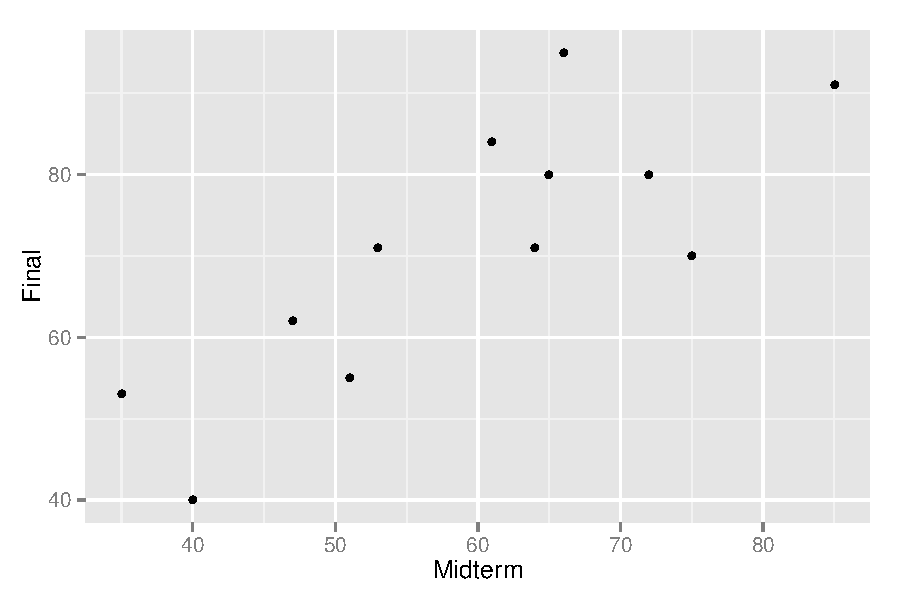
\includegraphics[scale = 0.5]{figures/exams_scatter.pdf}
    \caption{Questions \ref{q:exams.first}-\ref{q:exams.last}}
    \label{fig:exams}
  \end{figure}

  \begin{questions}
    
    % \question
    %   \[
    %      x = \{ 1, 5, 8, 12 \}
    %   \]

    %   \begin{parts}
    %     \part[2] What is $\bar{x}$.

    %       \begin{solution}
    %         $\bar{x} = 6.5$
    %       \end{solution}

    %     \part[3] What is the expression for $s_x$?
    %       \begin{solution}
    %         \[
    %           s_x = \sqrt{\frac{(1 - 6.5)^2 + (5 - 6.5)^2 + (8 - 6.5)^2 
    %             + (12 - 6.5)^2}{3}}
    %         \]
    %       \end{solution}

    %   \end{parts}


    \question[3] Estimate the mean score on the final for people who scored more than
      60 on the midterm:
      \label{q:exams.first}

      \begin{enumerate}[(a)]
        \item about 70
        \item about 80
        \item about 90
      \end{enumerate}

      \begin{solution}
        The students who scored more than 60 on the midterm are the students in the
        top right quadrant of the graph.  The mean on the final for these
        students is about 80.
      \end{solution}

    \question[3] Estimate the correlation coefficient:
      \begin{enumerate}[(a)]
        \item about 0.5
        \item about 0.8
        \item about 0.99
      \end{enumerate}

      \begin{solution}
        0.5 would be a more widely dispersed cloud of points and 0.99 would be
        a nearly straight line.  The actual coefficient is around 0.8.
      \end{solution}

    \question
      \label{q:exams.last}
      \begin{parts}
        
        \part[8] Draw box plots for the midterm and final
          \label{q:exams_box}

          \begin{solution}
            \begin{figure}[H]
              \centering
              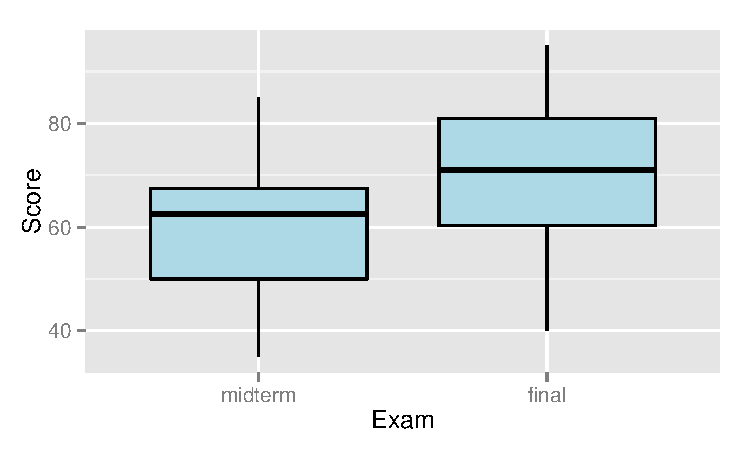
\includegraphics[scale = 0.6]{figures/exams_box.pdf}
              \caption{Question 3 (\ref{q:exams_box})}
              \label{fig:exams_box}
            \end{figure}
          \end{solution}

        \part[2] Compared to the midterm, was the final exam 
          \begin{enumerate}[(a)]
            \item harder 
            \item easier
            \item about the same difficulty
          \end{enumerate}

          \begin{solution}
            The scores were generally higher on the final, so the test was
            probably easier than the midterm.
          \end{solution}

      \end{parts}

    \question
      \label{q:point.histogram}
      Here are the average points per game for some NBA starting players:

      \begin{table}[ht]
        \centering
        \begin{tabular}{lr|lr}
          \toprule
          Player                   & Points & Player                 & Points\\
          \midrule
          Trey Burke               & 12.3   & LeBron James           & 27.2 \\
          Kentavious Caldwell-Pope & 6.0    & Michael Kidd-Gilchrist & 7.4 \\
          Tyson Chandler           & 9.3    & Robin Lopez            & 10.8 \\
          Glen Davis               & 12.1   & Kevin Martin           & 19.2 \\
          Jared Dudley             & 7.3    & Ben McLemore           & 7.6 \\
          Kevin Durant             & 31.8   & Chandler Parsons       & 16.6 \\
          Raymond Felton           & 10.0   & Kendrick Perkins       & 3.4 \\
          Randy Foye               & 12.6   & Zach Randolph          & 17.1 \\
          Marc Gasol               & 13.7   & Terrence Ross          & 10.7 \\
          Paul George              & 22.2   & Jared Sullinger        & 12.9 \\
          Spencer Hawes            & 13.0   & P.J. Tucker            & 9.3 \\
          Dwight Howard            & 18.9   & Evan Turner            & 16.6 \\
          \bottomrule
        \end{tabular}
        \caption{Points per game}.
      \end{table}

      \begin{parts}
        \part[10] Draw a histogram with a bin width of 5 points for these players.

        \begin{solution}
          Raymond Felton has an average of exactly 10, so you have a choice of
          what group to include him in.  I made the each bar include the lower
          boundary and exclude the upper boundary, but it is equally valid to do
          it the other way around also.

          Figure \ref{fig:point.histogram} contains the histogram.
        \end{solution}

        \ifprintanswers
          \begin{figure}[H]
            \centering
            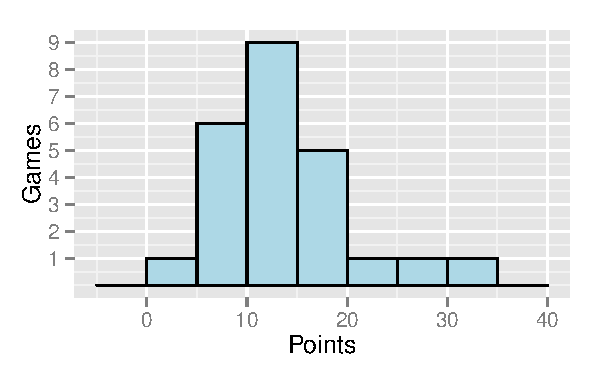
\includegraphics[scale = 1]{figures/point_histogram.pdf}
            \caption{Question \ref{q:point.histogram}}
            \label{fig:point.histogram}
          \end{figure}
        \fi

        \part[2] Is the distribution symmetrical, left-skewed, or right-skewed?
        \begin{solution}
          right-skewed
        \end{solution}

        \part[3] Is the mean larger or smaller than the median?  Explain how you
          can know the answer without calculating the actual values.
          \begin{solution}
            Because the distribution is right-skewed, the mean while be larger than
            the median.
          \end{solution}

        \part[3] Is the median or mean a better measure of the center of this
          distribution?  Why?

          \begin{solution}
            Since this is a skewed asymmetrical distribution, the median is a better
            measure of the center.  The median indicates what a typical player is
            likely to score, while the mean is heavily influenced by a few high
            scoring players.
          \end{solution}

      \end{parts}

    \question
      There is heated debate this year about whether Kevin Durant or
      LeBron James should be the MVP.  

      Here is a representative selection of the number of points they scored in
      selected games this season:

      \begin{tabular}[H]{ll}
        Durant & \{ 13, 17, 19, 24, 26, 28, 29, 31, 32, 32, 32, 37, 41, 42, 42 \} \\
        James  & \{ 13, 15, 17, 19, 25, 25, 25, 26, 29, 30, 32, 33, 35, 36, 36 \} \\ 
      \end{tabular}

      % \ifprintanswers
      %   \newpage
      % \fi

      \begin{parts}
        \part[8] Find the 5-number summary for both players
          \begin{solution}
            \begin{table}[H]
              \centering
              \begin{tabular}{lrrrrrr}
                \toprule
                Player & Min. & Q1 & Median & Q2 & Max. \\
                \midrule
                Durant & 13   & 24 & 31     & 37 & 42 \\
                James  & 13   & 19 & 26     & 33 & 36 \\
                \bottomrule
              \end{tabular}
            \end{table}

          \end{solution}

        \ifprintanswers
          \newpage
        \fi

        \part[6] Draw a box plot for both players
          \begin{solution}
            \begin{figure}[H]
              \centering
              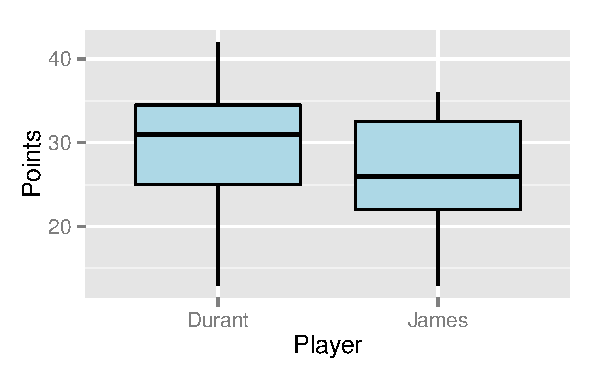
\includegraphics[scale = 0.7]{figures/james_vs_durant.pdf}
              \caption{James vs. Durant Points}
              \label{fig:james_vs_durant}
            \end{figure}
          \end{solution}

        % \ifprintanswers
        %   \newpage
        % \fi

        \part[3] Which player seems to be the MVP, based solely on points scored in
          these games? 
          \begin{solution}
            All of Durant's 5-number summary numbers except the minimum are
            better, and the minimum is the same.  The sample is representative
            of all the games.  If the award was based solely on scoring Durant
            would be the MVP.
          \end{solution}
      \end{parts}

      \question
        Three point shooting accuracy in 2013 is a roughly Normal distribution with a
        mean of 0.36 and a standard deviation of 0.05.

        \begin{parts}
          \part[5] Carmelo Anthony's three point shooting accuracy is 0.42 this
          year.  What is the z-score for this value?

          \begin{solution}
            \[
              \frac{0.42 - 0.36}{0.05} \approx \boxed{ 1.2 }
            \]
          \end{solution}

          \part[5] What percentage of the three point shooters in the NBA are less
            accurate than Melo?
            \begin{solution}
              If you look up Carmelo's z-score in table A, you find that about
              0.8849 or \fbox{ 88.5\% } of players have scores lower than 1.2.
            \end{solution}

          \part[5]
            What is the three point shooting accuracy for someone who is better
            than 20\% of the three point shooters?

            \begin{solution}
              For this problem you need to reverse the process.  From table A,
              the z-score that corresponds to $0.2$ is $-0.8416$.

              You have to convert this back to a shooting percentage:
              \begin{align*}
                -0.8416 & = \frac{x - 0.36}{0.05} \\
                x       & \approx \boxed{ 0.3179 } \\
              \end{align*}
            \end{solution}

        \end{parts}
        
      \ifprintanswers
      \else
        \newpage
      \fi

      \uplevel{
        Table \ref{tab:sbp} shows the shots made and missed by
            position for NBA players in the 2013-14 season.

        Use Table \ref{tab:sbp} to answer questions \ref{q:sbp.first}-\ref{q:sbp.last}.

        \begin{table}[H]
          \centering
          \begin{tabular}{lrr}
            \toprule
            position       & missed & made \\
            \midrule
            Center         & 11105  & 11372 \\
            Power Forward  & 18972  & 17601 \\
            Small Forward  & 19583  & 15090 \\
            Shooting Guard & 20721  & 15617 \\
            Point Guard    & 20791  & 15087 \\
            \bottomrule
          \end{tabular}
          \caption{Shots by position}
          \label{tab:sbp}
        \end{table}
      }

      \question[5] Make a bar plot showing shots made for each position.  Order
        the bars by number of shots made, with the most productive position first.
        \label{q:sbp.first}

        \begin{solution}
          \begin{figure}[H]
            \centering
            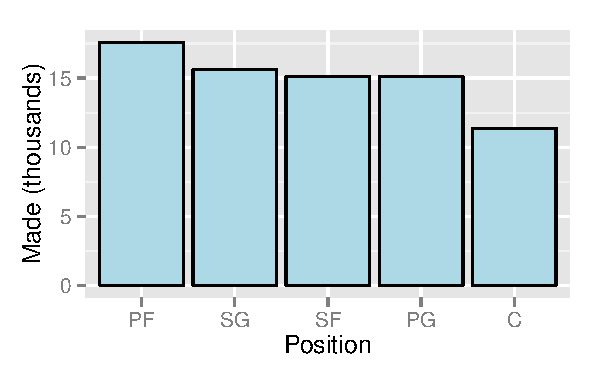
\includegraphics[scale = 0.8]{figures/shots_made.pdf}
            \caption{Question \ref{q:sbp.first}: shots made by position}
            \label{fig:sbp}
          \end{figure}

        \end{solution}
      \question[5] Fill in the table showing the marginal distributions of shots
      taken by position, shots missed, shots made, and total number of shots
      taken.

      \ifprintanswers
      \else
        \begin{table}[H]
          \centering
          \begin{tabular}{lrrr}
            \toprule
            position       & made  & missed & total \\
            \midrule
            Center         & 11372 & 11105  &       \\
            Power Forward  & 17601 & 18972  &       \\
            Small Forward  & 15087 & 20791  &       \\
            Shooting Guard & 15090 & 19583  &       \\
            Point Guard    & 15617 & 20721  &       \\
            \midrule
            total          &       &        &        \\
            \bottomrule
          \end{tabular}
          \caption{Marginal distributions}
          \label{tab:marginal_shots}
        \end{table}
      \fi

      \begin{solution}
        
        \begin{table}[H]
          \centering
          \begin{tabular}{lrrr}
            \toprule
            position       & made  & missed & total \\
            \midrule
            Center         & 11372 & 11105  & 22477 \\
            Power Forward  & 17601 & 18972  & 36573 \\
            Small Forward  & 15087 & 20791  & 35878 \\
            Shooting Guard & 15090 & 19583 & 34673 \\
            Point Guard    & 15617 & 20721 & 36338 \\
            \midrule
            total          & 74767 & 91172 & 165939 \\
            \bottomrule
          \end{tabular}
          \caption{Marginal distributions}
          \label{tab:marginal_shots}
        \end{table}

      \end{solution}

      \question 
        \label{q:sbp.last}
        \begin{parts}
          \part[5] Make a table showing the conditional distributions of percentage
          of shots made and missed for each position.  

          \begin{solution}
            \begin{table}[H]
              \centering
              \begin{tabular}{rlrr}
                \toprule
                position       & made & missed \\
                \midrule
                Center         & 51\% & 49\% \\
                Power Forward  & 48\% & 52\% \\
                Small Forward  & 44\% & 56\% \\
                Shooting Guard & 43\% & 57\% \\
                Point Guard    & 42\% & 58\% \\
                \bottomrule
              \end{tabular}
            \end{table}
          \end{solution}

          \part[2] Which position seems to contain the most accurate shooters?
            Is this is because they are the best shooters or is there a lurking
            variable that explains the shooting percentage differences?
          
            \begin{solution}
              The centers are the most accurate shooters. This is because most
              of them are 7 feet tall and never venture more than 3 feet from
              the basket or attempt a shot more difficult than a dunk.
            \end{solution}

        \end{parts}
      
      \ifprintanswers
      \else
        \newpage
      \fi

      \question
        \label{q:draft}

        \begin{figure}[H]
          \centering
          \ifprintanswers
            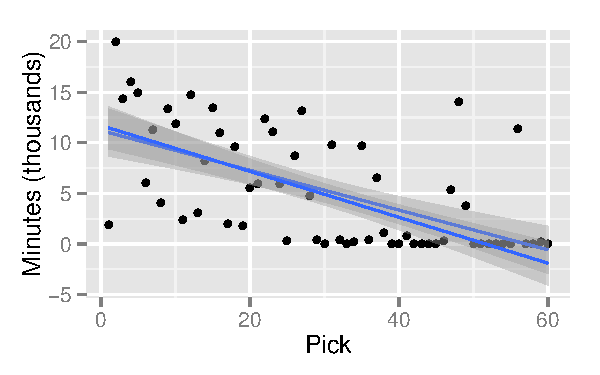
\includegraphics[scale = 0.8]{figures/draft_with_regression.pdf}
          \else
            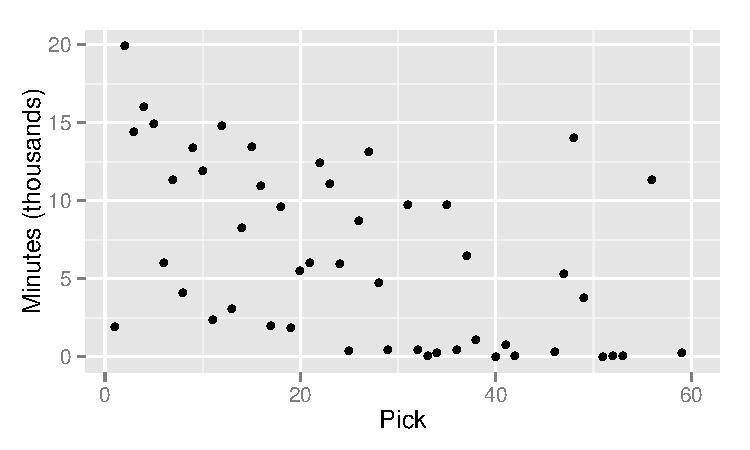
\includegraphics[scale = 0.8]{figures/draft.pdf}
          \fi
          \caption{2008 NBA draft order vs. minutes played}
          \label{fig:draft}
        \end{figure}

        \begin{table}[H]
          \centering
          \begin{tabular}{lrr}
            \toprule
                                & mean & s \\
            \midrule
            Pick                & 30.5 & 17.5 \\
            Minutes (thousands) & 5219 & 5698 \\
            \bottomrule
          \end{tabular}
          \caption{2008 NBA Draft}
        \end{table}

        Figure \ref{fig:draft} shows the total number of minutes played vs.  draft
        order for the 2008 draft.  The better players are generally drafted first
        and also usually play more, so there is a negative correlation of 
        $r = -0.6020$ between draft order and minutes played.

        The first two selections in the 2008 draft were Greg Oden (bottom left
        corner) and Kevin Durant (top left corner).  As you can see in the
        chart, Greg Oden has had an injury plagued career and has only played
        1940 minutes while Kevin Durant has had a successful and so far mostly
        injury free career and has played nearly 20,000 minutes

        Many of the players after pick 30 never played in the NBA at all.  Any
        of them that were underclassmen declaring for the draft early should
        have stayed in school.

      \begin{parts}
        \part[7]
          Find the equation for the regression line using the draft pick as the
          explanatory variable and minutes played as the response variable.  
          \begin{solution}
            Use the correlation coefficient and the standard deviations to find
            the slope of the regression line:
            \[
              b = -0.6020 \cdot \frac{5698}{17.5} \approx -196
            \]

            Use the slope and the means to find the y-intercept:
            \begin{align*}
              \bar{y} & = a - 196 \bar{x} \\
              5219    & = a - 196 \cdot 30.5  \\
              a       & \approx 11,197 \\
            \end{align*}

            The equation is:
            \[
              \boxed{ \hat{y} = 11,197 - 196 x }
            \]

          \end{solution}
        \part[5] Graph the regression line.
        \begin{solution}
          See Figure \ref{fig:draft} (slightly less steep regression line).
        \end{solution}

        \ifprintanswers
          \newpage
        \fi

        \part[2] What percentage of the variation in the minutes played is
          accounted for by the linear regression line?

          \begin{solution}
            $r^2 \approx 0.3625$
          \end{solution}

        \part[3] Mark Gasol and Ramon Sessions (top right corner) are outliers
        because they were late round draft picks (pick 48 and 56) who have had a
        successful NBA careers with over 11,000 minutes each so far.

        Would removing these data points from the graph have a significant
        effect on the regression line?  Why or why not? 

        \begin{solution}
          It depends on what you mean by ``significant.''  You could say ``yes''
          because they are away from the center of the graph, so they are sort
          of outliers on the x axis.  On the other hand, you could say ``no''
          because there are 7 other points in the same x-range right around
          zero, so the line can't follow the outliers very well.  

          Either answer is correct, as long as you provided a reasonable
          explanation.

          The actual numbers without those two players are:
          \begin{align*}
            r       & \approx -0.6975 \\
            \hat{y} & \approx 11,708 -227 x \\
          \end{align*}

          Both regression lines are in Figure \ref{fig:draft}.  The line without
          the outliers is slightly steeper (lower on the right side).
        \end{solution}
      \end{parts}


  \end{questions}
\end{document}

